\documentclass[tikz]{standalone}

\usepackage{tikz}
\usetikzlibrary{trees}
\usetikzlibrary{shapes}
\usetikzlibrary{positioning}
\usetikzlibrary{arrows.meta}

\tikzset{
    pointer/.style = {thick,draw=black,triangle 45-*,shorten >=-3pt},
    cell/.style = {rectangle, thick, draw=black,minimum width = 1cm, minimum height =1.0cm,fill=yellow!20},
    mynode/.style = {circle, thick, draw=black, align=center,fill=yellow!40,font=\ttfamily\bfseries\Large},
    mynoder/.style = {circle, thick, draw=black, align=center,fill=red!30,font=\ttfamily\bfseries\Large},
    mynodeb/.style = {circle, thick, draw=black, align=center,fill=blue!30,font=\ttfamily\bfseries\Large},
    edgen/.style = {-latex,ultra thick},
    edger/.style = {-latex,ultra thick,red},
    edgeb/.style = {-latex,ultra thick,blue},
    edgeg/.style = {-latex,ultra thick,gray},
    edgegd/.style = {-latex,ultra thick,brown,dashed}, % back
    edgevd/.style = {-latex,ultra thick,violet,dotted}, % forward
    edgexd/.style = {-latex,ultra thick,blue,densely dotted}, % traversal
    every picture/.style={/utils/exec={\ttfamily\bfseries}},
    every picture/.style={font issue=\ttfamily\bfseries},
    font issue/.style={execute at begin picture={#1\selectfont}
  }
}

\begin{document}
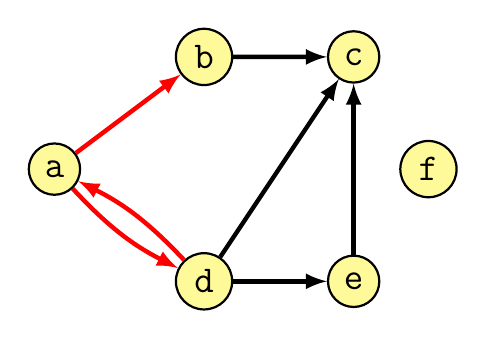
\begin{tikzpicture}[scale=0.95,transform shape]
%
\node[mynode] at (0,0) (a) {a};
\node[mynode] at (2,1.5) (b) {b};
\node[mynode] at (4,1.5) (c) {c};
\node[mynode] at (2,-1.5) (d) {d};
\node[mynode] at (4,-1.5) (e) {e};
\node[mynode] at (5,0) (f) {f};
%
\draw[edger] (a) edge node {} (b);
\draw[edger] (d) edge[bend right=10] node {} (a);
\draw[edger] (a) edge[bend right=10] node {} (d);
\draw[edgen] (b) edge node {} (c);
\draw[edgen] (d) edge node {} (c);
\draw[edgen] (d) edge node {} (e);
\draw[edgen] (e) edge node {} (c);
\end{tikzpicture}
\end{document}